\newpage
\section{Test 6}
\label{Sec:test_6}

In the sixth test setting rover is dropped onto the horizontal plane from the height of $2$ $m$. After $10$ $s$ linearly varying torques are applied to all wheels. 
A spherical obstacle has been set in front of the rover. The obstacle is in the form of a sphere which protudes outside the plane.
Center of the sphere has been set so that the protrusion is equal to $20$ $cm$. Coefficient of friction has been set to 0.3 whereas the coefficient of restitution to 0.

\begin{figure}[H]
  \centering
    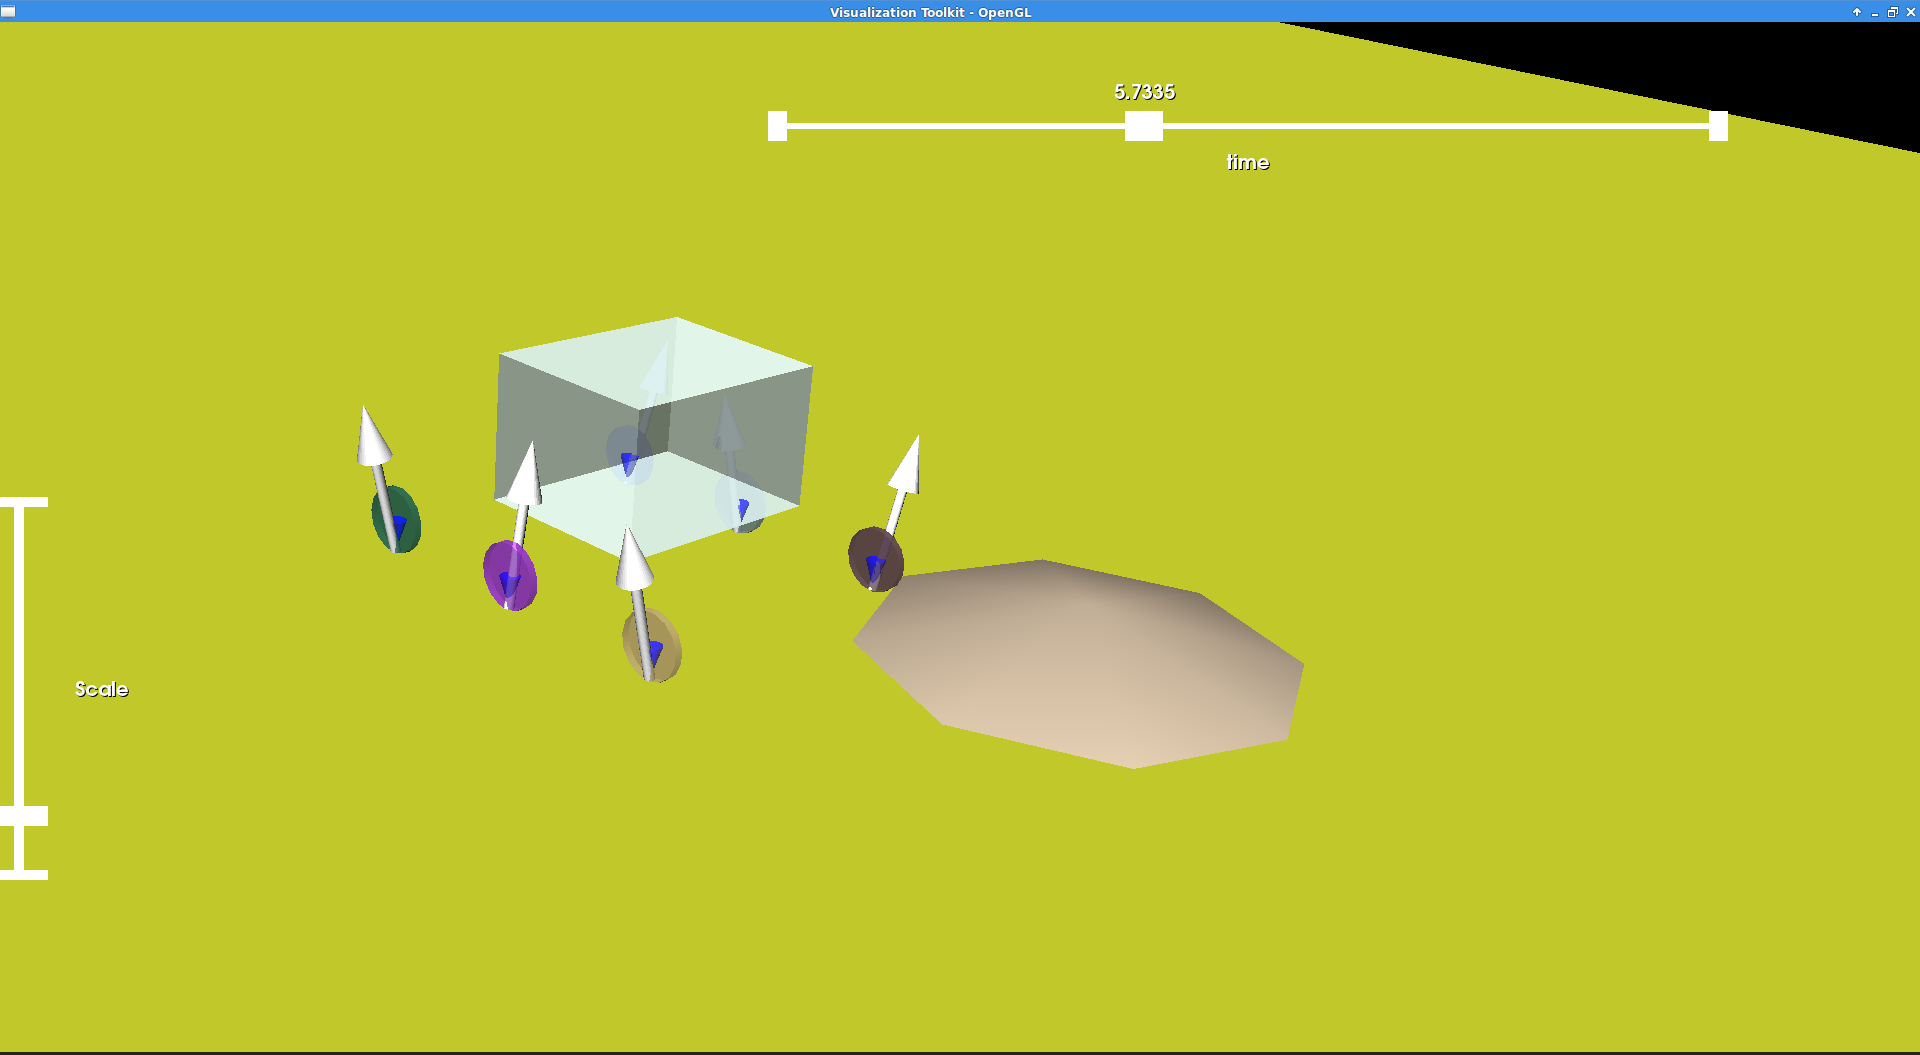
\includegraphics[width=0.8\textwidth]{run_6}
  \caption{Sixth test scenario}
\end{figure}

\noindent In this case, the following essential quantities have been plotted:

\begin{figure}[H]
  \centering
    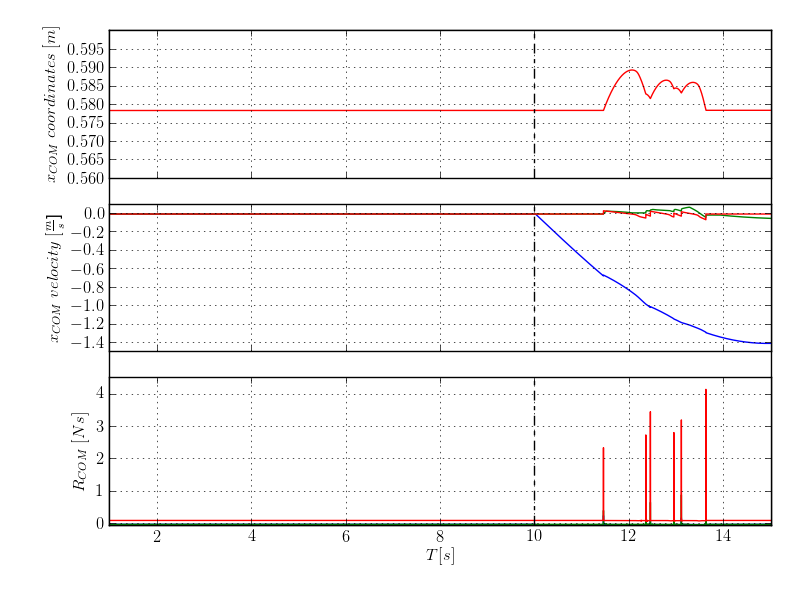
\includegraphics[width=0.8\textwidth]{xvpCOM6}
  \caption{position, velocity and reaction forces of the mass center of the rover}
\end{figure}

\noindent \textbf{\textit{\Large{Comments}}}\\[1mm]
\noindent In this setting attention can be drawn to the spherical obstacle crossing. In the figure 27 in the first sub-plot on can see $z$ coordinate evolution of the mass center of the robot. 
It is clearly seen how around 11$^{th}$ minute rover mounts the sphere. In the sub-plot below one can see the evolution of velocities of the mass center where several small jumps occur in the 
$y$ and $z$ dimension as a result of impacts. Velocity in the $x$ direction is clearly larger as the rover moves along the $x$ axis. Impacts are more clearly seen in the third sub-plot with each peak 
corresponding to an impact.\\
 
\noindent Following additional quantities have also been plotted:

\begin{figure}[H]
  \centering
    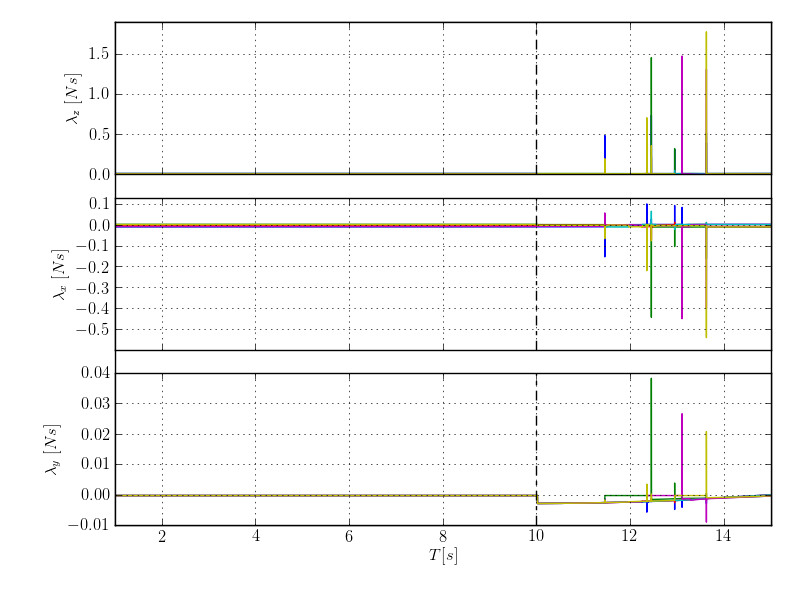
\includegraphics[width=0.8\textwidth]{lambdaNTS6}
  \caption{$\lambda_{N}$, $\lambda_{T_x}$, $\lambda_{T_y}$ - normal component of the contact force (impulsion) for each wheel (interaction with the plane)}
\end{figure}

\begin{figure}[H]
  \centering
    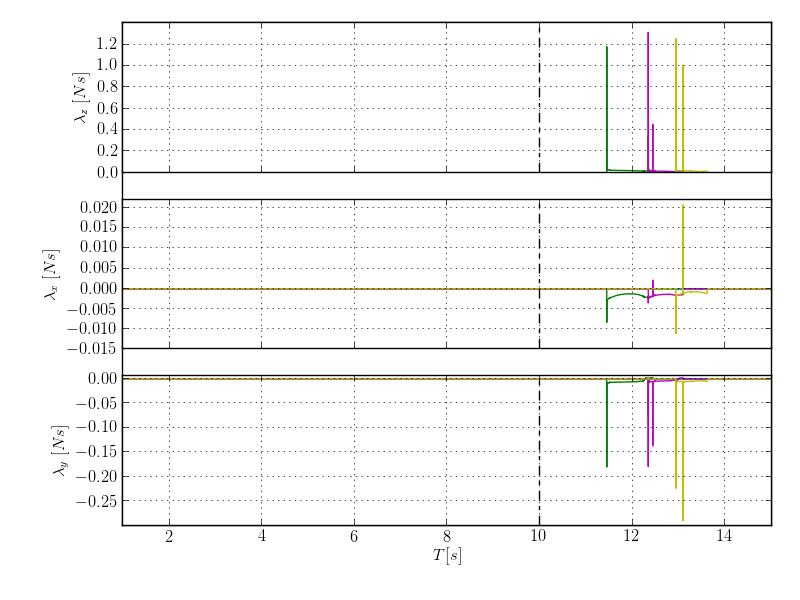
\includegraphics[width=0.8\textwidth]{lambdaNTS6sphere}
  \caption{$\lambda_{N}$, $\lambda_{T_x}$, $\lambda_{T_y}$ - normal component of the contact force (impulsion) for each wheel (interaction with the sphere)}
\end{figure}

\noindent \textbf{\textit{\Large{Comments}}}\\[1mm]
\noindent In the figure 28 and 29 local contact forces have been plotted seen from the interaction with plane and sphere respectively. One can observe several peaks corresponding to the
phase of the simulation when the obstacle is being crossed.\\
